\documentclass[11pt, oneside]{article}   	% use "amsart" instead of "article" for AMSLaTeX format
\usepackage{geometry}                		% See geometry.pdf to learn the layout options. There are lots.
\geometry{letterpaper}                   		% ... or a4paper or a5paper or ... 
%\geometry{landscape}                		% Activate for rotated page geometry
%\usepackage[parfill]{parskip}    		% Activate to begin paragraphs with an empty line rather than an indent
\usepackage{graphicx}				% Use pdf, png, jpg, or eps§ with pdflatex; use eps in DVI mode
								% TeX will automatically convert eps --> pdf in pdflatex		
\usepackage{amssymb}
\usepackage{url}

%SetFonts

%SetFonts


\title{Self-regulation ontology project: Sampling simulations}
\author{Russell Poldrack, with help from Dave Mackinnon and Oscar Gonzales}
%\date{}							% Activate to display a given date or no date

\begin{document}
\maketitle
\section{Introduction}
At the kickoff meeting for this project on Nov 23, 2015, there was discussion regarding the most optimal sampling schemes for the proposed study.  The goal of this document is to lay out the work done to assess the questions raised in this discussion.

The original sampling plan was to attempt to enroll a number of MTurk workers to complete the entire battery of tasks (currently estimated at about 70 tasks).  This has the benefit of providing a relatively large number of subjects with substantial coverage of the full battery across ~ 10 sessions, but it also raises practical concerns.  In particular, the rate of attrition to be expected from this procedure is currently unknown, and a  high rate of non-completion of the full battery would raise difficult modeling issues, because the data would be missing not at random.  Dave Mackinnon suggested that it might be more optimal to instead sample a larger number of indviduals on a smaller portion of the battery using random assignment of tests to subjects, so that missing data would be missing completely at random, which allows the use of a much wider and more convenient set of modeling tools.  At the meeting it was decided that simulations were in order to assess this question.

\section{Simulation methods}
Simulations were based on real data obtained from the UCLA Consortium for Neuropsychiatric Phenomics (CNP).  This dataset consists of 1254 subjects studied across a large number of measures.  We selected a subset of 36 summary measures for further examination, including both performance and questionnaire measures relevant to the proposed work; The total number of complete cases across these measures was 1093.  

The data were first submitted to exploratory factor analysis in order to identify the veridical factor structure for the dataset.  There was no clear answer for the optimal number of factors.  Parallel analysis (using fa.parallel() in the R psych package) suggested that the optimal number of factors was 8. Very Simple Structure analysis (using the vss() function in the psych package) suggested 9 factors by the BIC criterion and 12  by the sample-size adjusted BIC criterion, whereas VSS complexity criteria suggested fewer structures (4 and 6 for VSS complexity critieria 1 and 2 respectively).  Based on these analyses a dimensionality of 9 factors was chosen for exploratory factor analysis (EFA).  

Three confirmatory factor analysis (CFA) models were generated based on the results from the EFA.  The first (veridical model) was generated based on the actual structure obtained from EFA applied to the full dataset; links were included for all variables with loading of at least 0.1 on each factor in the original EFA.  The second was a slight modification of the first, obtained by dropping one variable from one factor, and the third was a greater modification obtained by collapsing two factors from the original model into a single factor.  Each of these fit the data significantly worse than the veridical model (model 2: $\chi^2$= 20.13; model 3: $\chi^2$= 145.77, both $p<0.001$).


These models are presented in Figure \ref{fig:models}.

\begin{figure}[!h]
\caption{\textbf{Correct CFA Model 1 (left) and incorrect (CFA) models 2 (close - missing one link) and 3 (far - factors H and I combined).}}
\centering
\includegraphics[width=1.\linewidth]{models.pdf}
\label{fig:models}
\end{figure}

Simulated datasets were generated by sampling subjects with replacement from the original 1093.  The base sample size for the simulations was varied between 400 and 800 subjects (in steps of 100), which was used for simulations with complete cases (no missing data).  Datasets with missing data were generated by sampling larger datasets and then setting a particular proportion of variables to NA for each subject; the sample size was increased in order to keep the total number of non-NA cells constant across simulations.  

The three CFA models were fit to each simulated dataset using the lavaan package in R. We initially explored the use of imputation with the Amelia II package, but overimputation analysis showed very poor fit between imputed and actual data, so this approach was not examined in detail for the full simulations.  Instead, models were fit using full information maximum likelihood (FIML) with no imputation (which is appropriate given that the data are missing completely at random); a fairly high ridge parameter (ridge=0.1) was used to help prevent degeneracies in model fitting.  The primary measures of interest were root mean square approximation error (RMSEA) which is a measure of goodness of fit of the correct model, and the p-value for the model comparison between the correct model and two incorrect models, which was used to estimate statistical power to distinguish correct vs. incorrect models.  For each model, 500 simulations were run for multiple levels of sampling (36, 18, 9, 6, 4, and 3 of the 36 tasks present for each subject); see \url{https://github.com/poldrack/SEM_simulations/blob/master/SEM_sim2.R}.

\section{Results}

Results of the simulations are presented in Figure \ref{fig:results}.  An important finding was that model fitting failed regularly, with increasing rates of failure as the amount of missing data increased (Figure \ref{fig:results}C); this is likely due to ill-conditioned (non-positive definite) covariance matrices obtained from the missing data, or from small numbers of observations for particular combinations of variables.   With small sample sizes and low sampling per subject, nearly all modeling attempts were unsuccessful.  All subsequent analyses are conditionalized upon successful model fitting.

Model fit and power to detect close and far model misspecification were examined at each base sample size (400-800 in steps of 100) for each level of test sampling.  Results are presented in Figure \ref{fig:results}.  Model goodness of fit was strongly modulated by sampling (Figure \ref{fig:results}A), which likely reflects the fact that RMSEA is sensitive to sample size, and sample size increased as the number of variables sampled per individual decreased (in order to keep the number of complete cells constant).  Far model misspecfication was easily detected (not shown); for most simulations power was 100\%, and it was only for base sample size of 400 with 3 tests sampled that it fell below 80\%.  Close model misspecfication was more difficult to detect (Figure \ref{fig:results}B); for no set of simulations was power greater than 80\% to detect the misspecification of a single variable, though it approached 80\% for the simulations with all 36 variables.  Pilot analyses had identified cases where an RMSEA value of zero was returned, which presumably reflected some sort of degeneracy in model fitting.  In the present simulations this was only observed for analyses with very small numbers of variables present (Figure \ref{fig:results}D).  


\begin{figure}[!h]
\caption{\textbf{Results from simulations}}
\centering
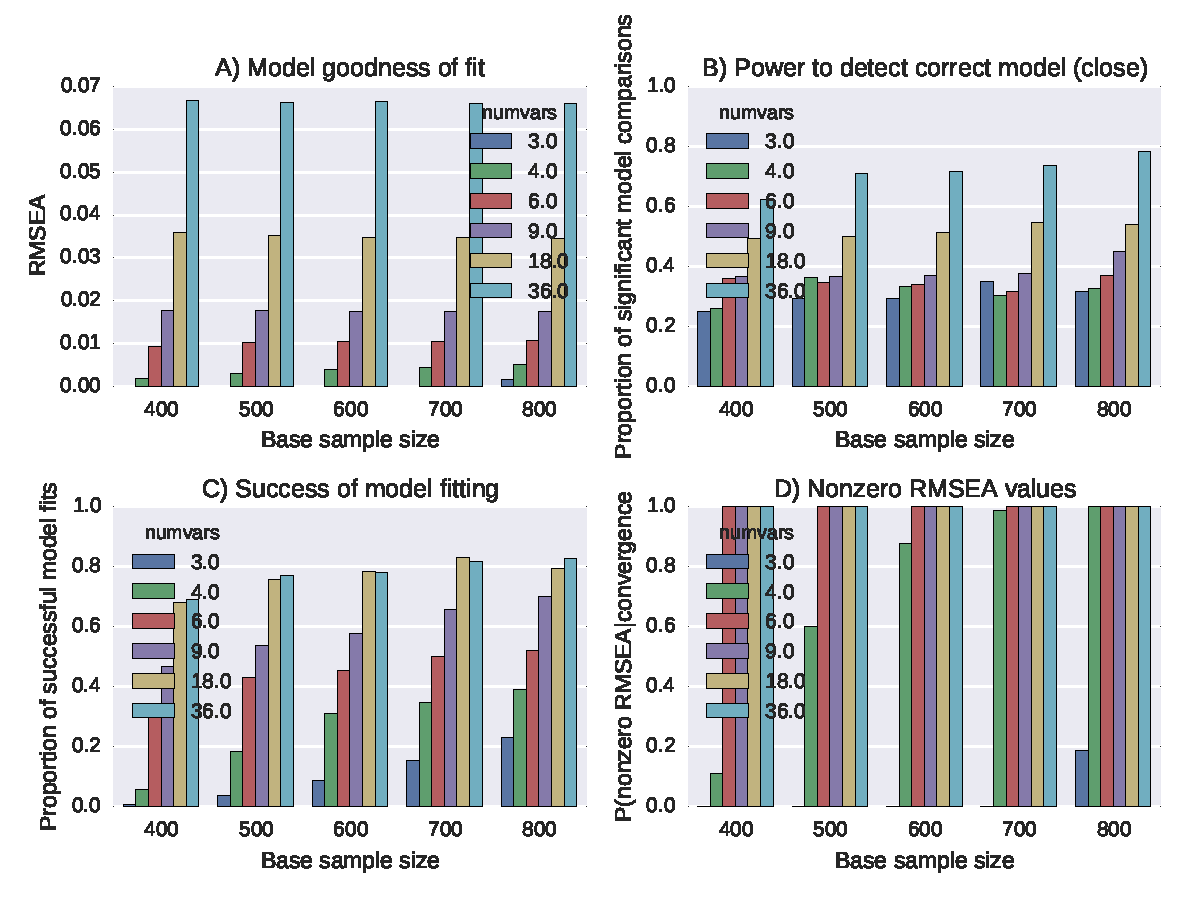
\includegraphics[width=1.\linewidth]{results_power.pdf}
\label{fig:results}
\end{figure}

\section{Summary}
The foregoing results provide some guidelines regarding the sampling of measures in the proposed study.  In particular, they suggest that subsampling of individuals across measures is a reasonable approach that may help balance the logistical challenges of sampling individuals across a large number of measures.  They also provide some practical limits on this subsampling, suggesting that each individual should probably be sampled in such a way as to provide data on at least about 1/6 of the measures in the database.  One limitation of the present work is that we don't know how it will scale to an even larger set of measures like those in the proposed study; it would be possible to assess this using simulated data once the full set of variables is known.

The results also suggest a strategy for sampling of measures; in particular, we should sample measures in such a way as to prevent substantial imbalances in the number of observations for each pairwise set of variables.  This could be achieved by randomly sampling subsets of measures for each new subject, with sampling driven by the observed frequencies in the joint histogram across measures (see Figure \ref{fig:sampling}); for an example implementation, see \url{https://github.com/poldrack/SEM_simulations/blob/master/sampsim.py}.

\begin{figure}[!h]
\caption{Simulation of test sampling, showing that random sampling can result in some sets of measures with very low numbers of pairwise datasets (total number of tests = 70, number assigned to each subject = 12, number of subjects = 4000).  Subjects were either randomly assigned to tests (blue line), or assigned to tests by choosing the tests with the lowest joint frequencies in the histogram (green line).  The minimum cooccurrence frequency was substantially higher for the optimal sampling (103) versus the random sampling (74)}
\centering
\includegraphics[width=1.\linewidth]{optsample.pdf}
\label{fig:sampling}
\end{figure}

%The one major remaining concern is the high degree of model fitting failure; even in the complete case simulations there was more than 10\% failure of model fitting, and this increased to almost 80\% modeling failure rate in the case with 80\% of values missing, both for FIML and for imputation using Amelia.  It would be useful to gain more insight into these failures so that we can avoid a case where our proposed models cannot be fit. 


\end{document}  